% Preamble.
\documentclass{article}

\title{Programming Project 5}
\author{Max Reilly, copied from Hanly and Koffman}
\date{April 4, 2024}

\usepackage{pdfpages}
\usepackage{graphicx}

\begin{document}
\maketitle
\section{Assignment}
In this chapter we studied the bisection method for finding a root of an equation. Another method of
finding a root, Newton's method, usually converges to a solution even faster than the bisection
method, if it converges at all. Newton's method starts with an initial guess for a root $x_0$, and
then generates successive approximate roots $x_1, x_2, . . . , x_j, x_{j+1} . . .$ using the iterative
formula

$$
x_{j+1} = x_j - \frac{f(x_j)}{f'(x_j)}
$$

where $f'(x_j)$ is the derivative of function $f$ evaluated at $x = x_j$. The formula generates a new
guess, $x_{j+1}$, from the previous one, $x_{j}$. Sometimes Newton's method will fail to converge to
a root. In this case, the program should terminate after many trials, perhaps 100.

Figure 7.12 shows the geometric interpretation of Newton's method where $x_0$, $x_1$, and $x_2$
represent successive guesses for the root. At each point $x_j$, the derivative, $f'(x_j)$, is the
slope of the tangent to the curve, $f(x)$. the next guess for the root, $x_{j+1}$, is the point at
which the tangent crosses the x axis.

for geometry, we get the equation

$$
\frac{y_{j+1} - y_j}{x_{j+1} - x_j} = m
$$

% 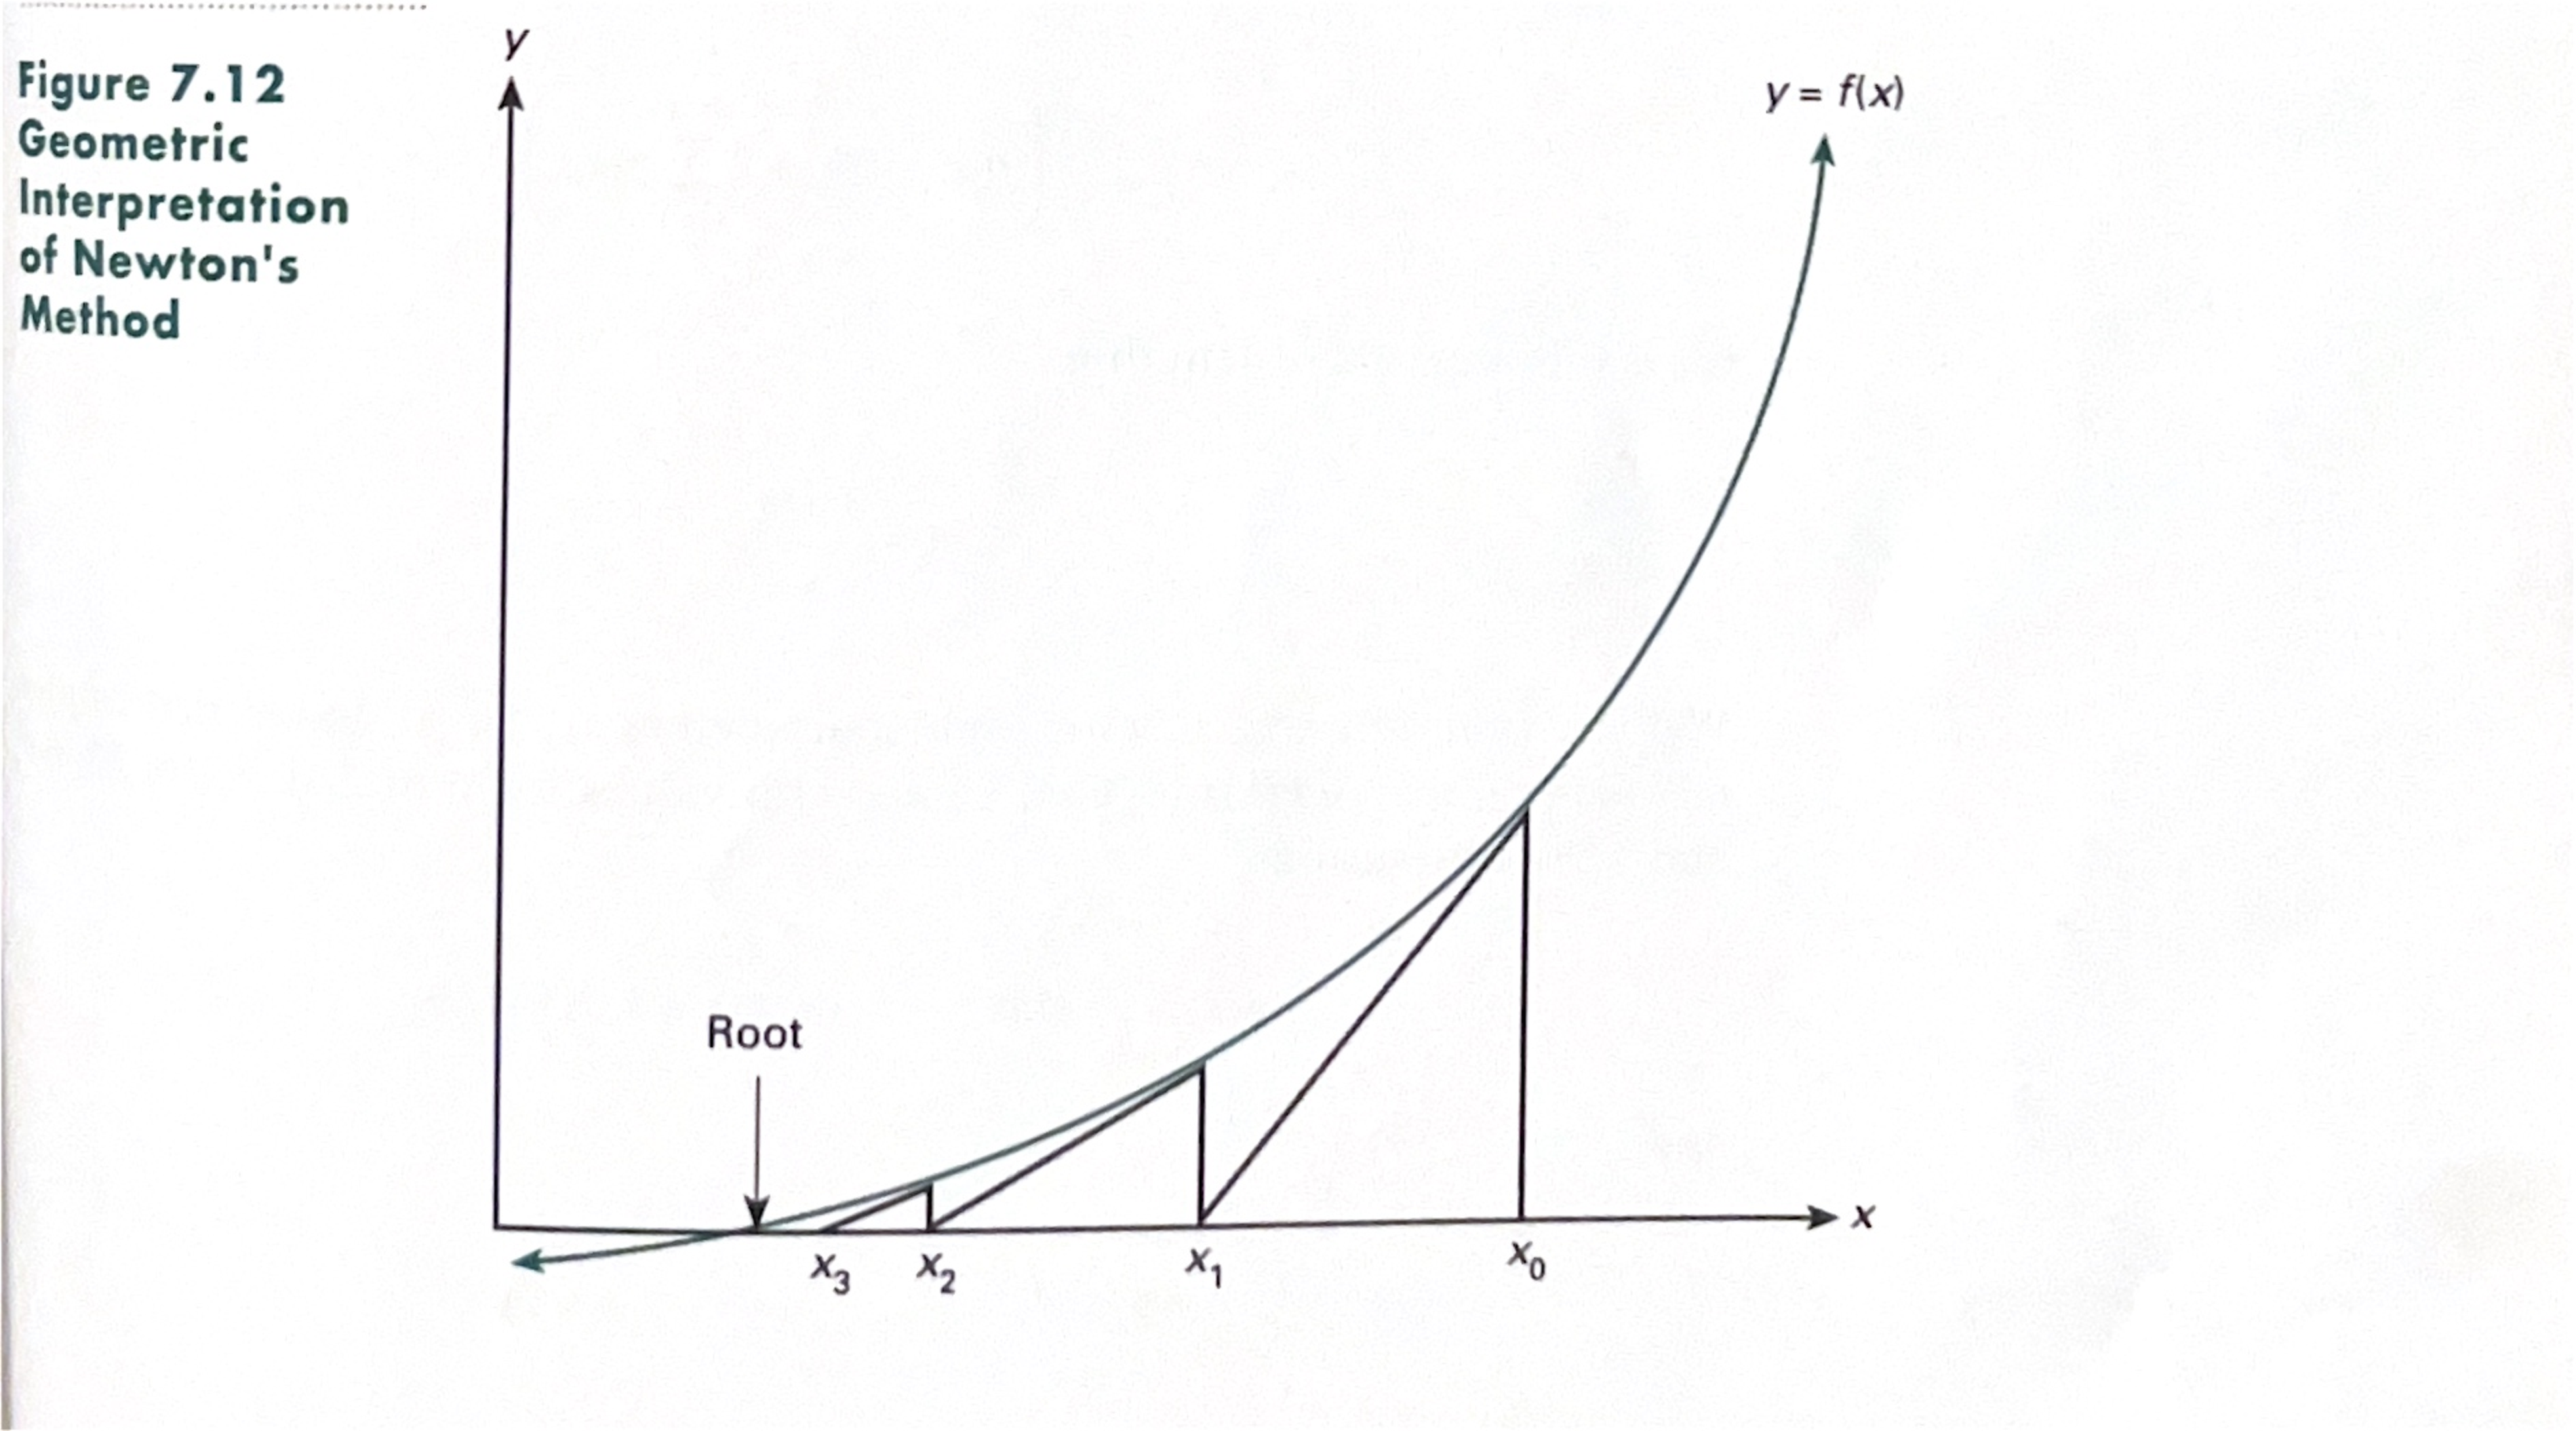
\includegraphics{hk_fig_7.12.pdf}
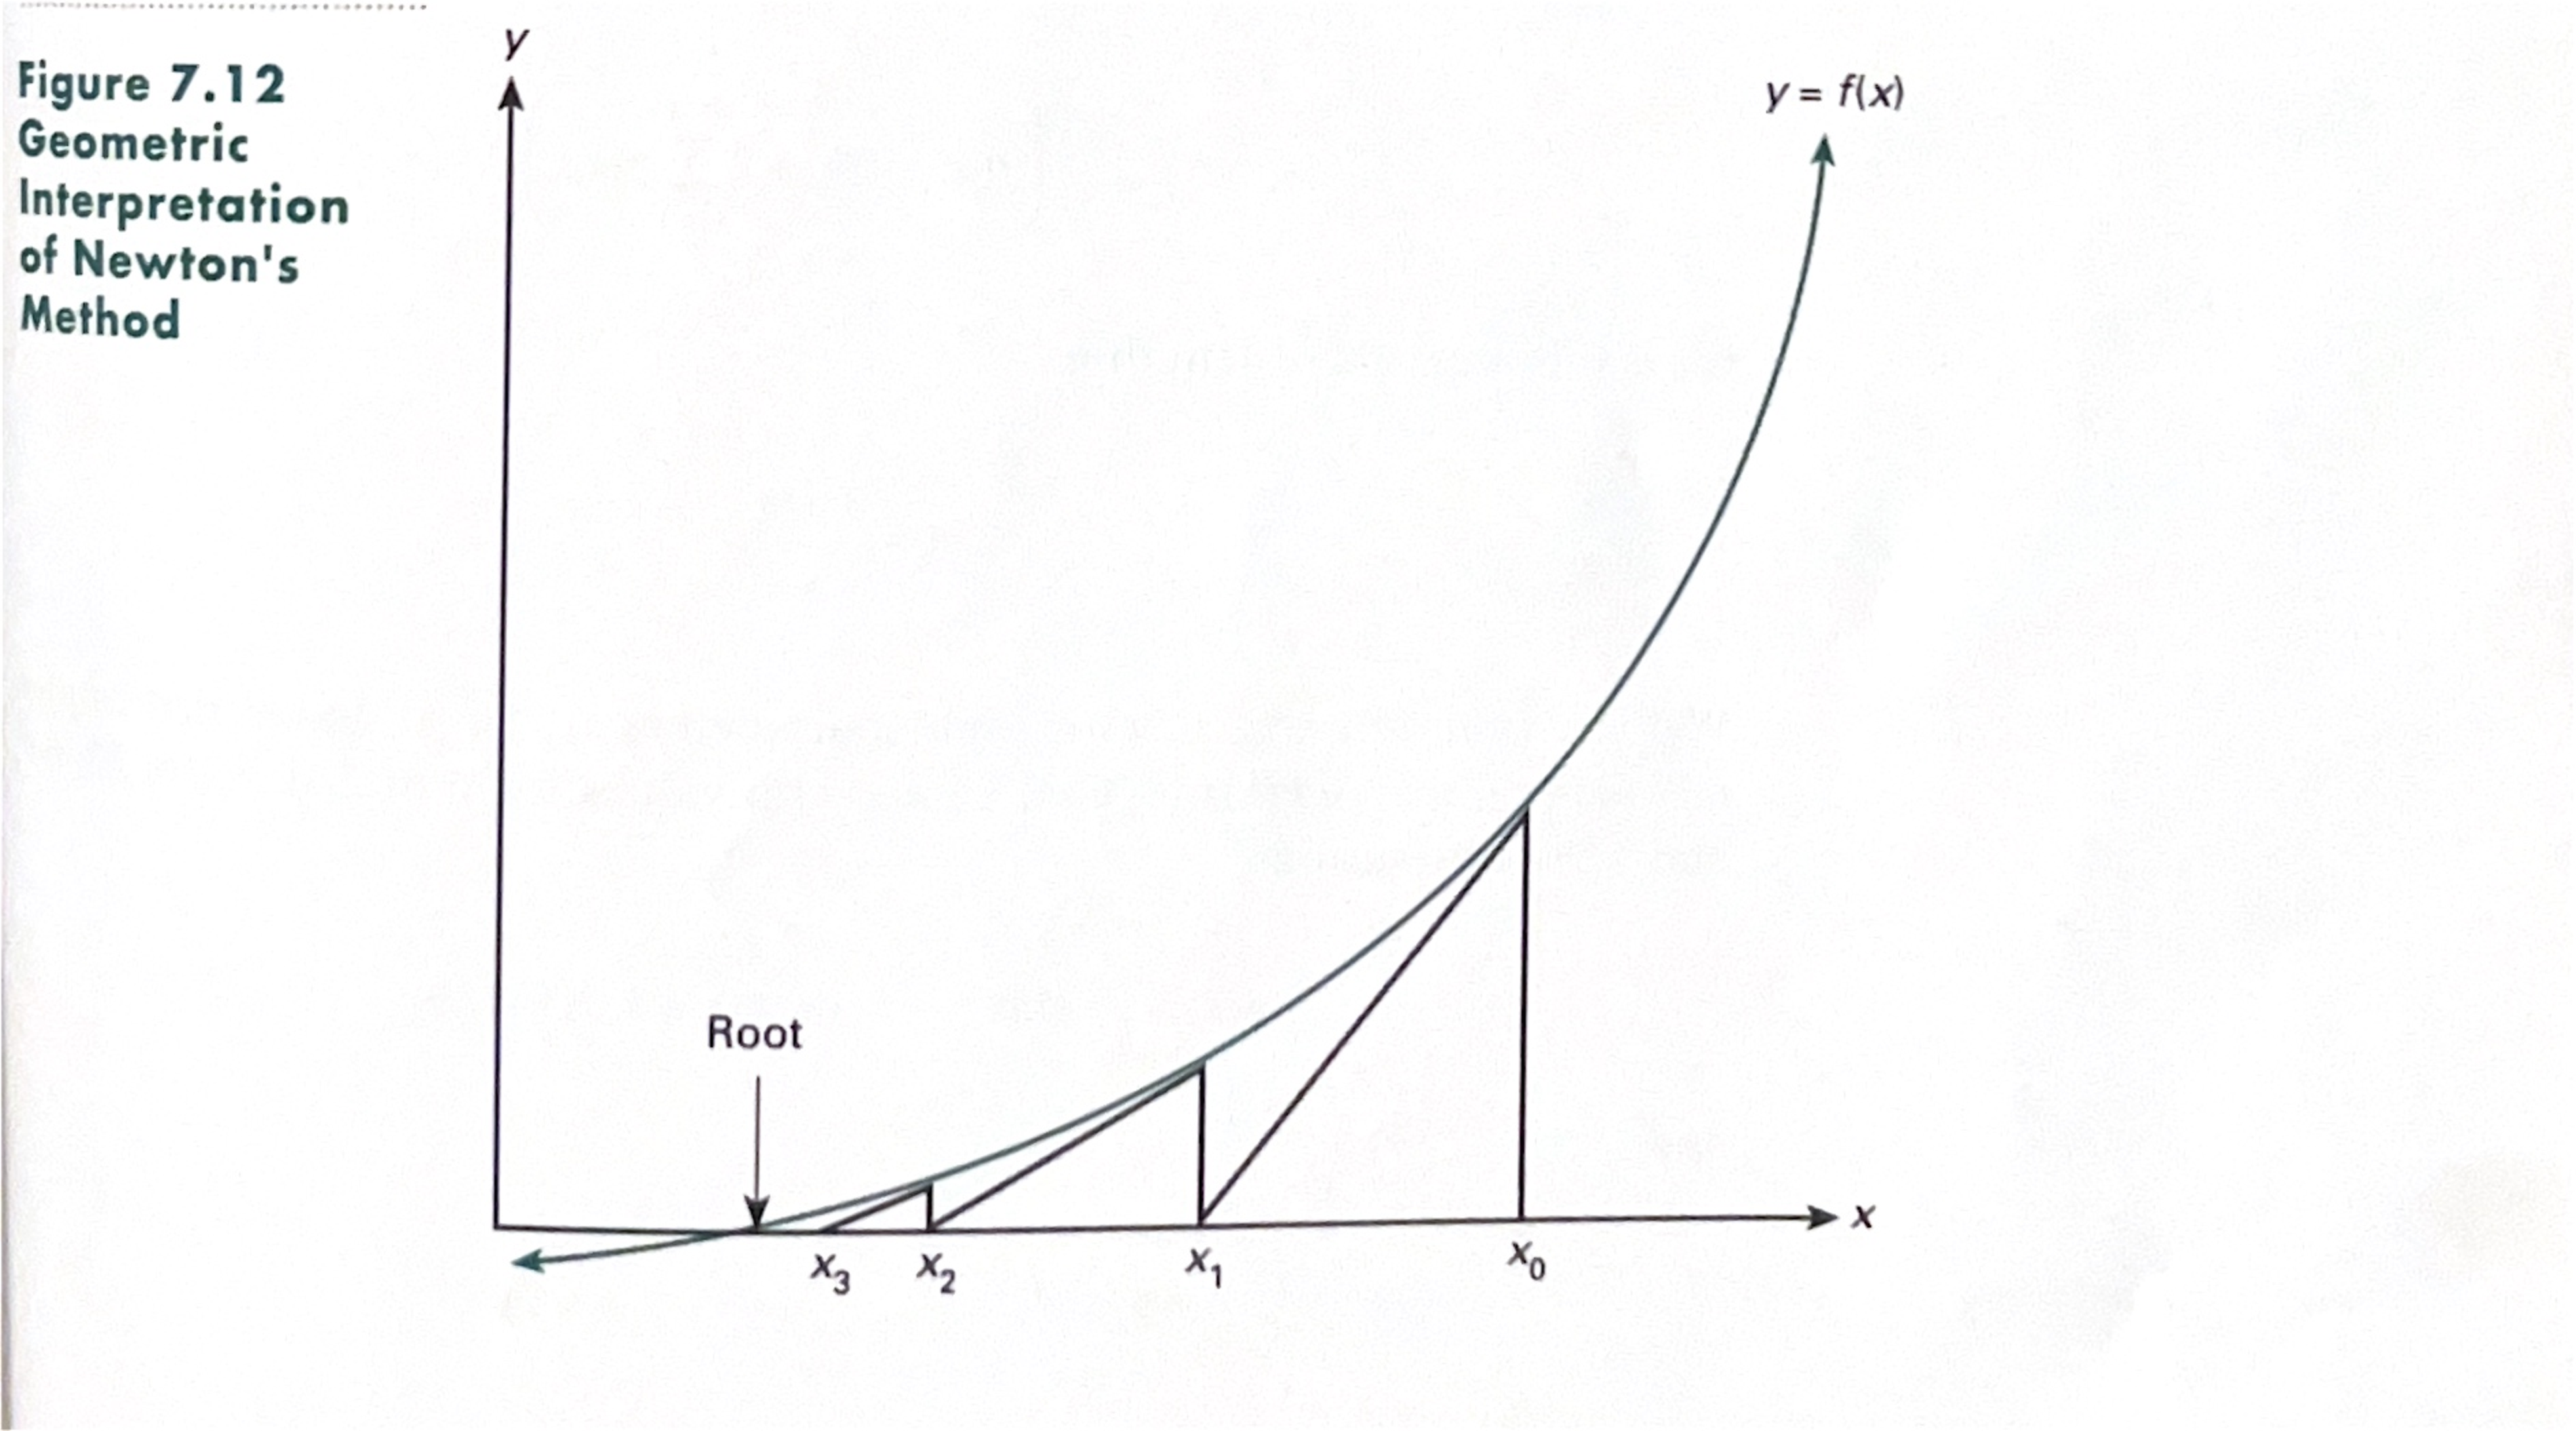
\includepdf[pages=-]{hk_fig_7.12.pdf}
Where $m$ is the slope of the line between points $(x_{j+1}, y_{j+1})$ and $(x_j, y_j$. In Fig 7.12,
we see that $y_{j+1}$ is zero, $y_j$ is $f(x_j)$, and $m$ is $f'(x_j)$; therfore by substituting and
rearranging terms, we get

$$
-f(x_j) = f'(x_j) \times (x_{j+1} - x_j)
$$

leading to the formula shown at the beginning of this problem.

Write a program that uses Newton's method to approximate the nth root of a number to six decimal
places. If $x^n = c$, then $x^n -c = 0$. Finding a root of the second equation will give you
$\sqrt[n]{c}$. Test your program on $\sqrt{2}$, $\sqrt[3]{7}$, and $\sqrt[3]{-1}$. Your program could
use $c/2$ as it's initial guess.

\section{Notes}
\begin{itemize}
    \item It occurs to me, it might be better to start making these notes simply in latex, since I am
            trying to get better with that anyway. Might be a fun and easy way to get what I want!
\end{itemize}

\end{document}
